\chapter{Protein-protein Interaction Prediction: SPRINT}
This chapter descibes two of our publications SPRINT \cite{li2017sprint, li2020predicting}, a sequence based protein-protein interaction site prediction program. We first introduce the prerequisites used in SPRINT as well as the state-of-the-art methods. Then we describe both the algorithm and the implementation of SPRINT in details.  Last, we compare DELPHI with five state-of-the-art programs on seven datasets showing that it is more accurate while running orders of magnitude faster and using very little memory.
\section{Background}
\subsection{Basic Notions and Definitions}
\subsubsection{BLAST seeds}
\subsubsection{Spaced seeds}
\subsubsection{Multiple spaced seeds}
\subsubsection{Substitution matrix}
\subsubsection{Interactome prediction}
\subsection{Previous Methods}
As shown in Table \ref{table_experimental_ppi_pred}, various experimental techniques for identifying PPIs have been developed, most notably high throughput procedures such as two-hybrid assay and affinity systems \cite{shoemaker2007deciphering}. Such methods are time and labor intensive and have a high rate of error. Therefore, a variety of computational methods have been designed to help predicting PPIs, employing sequence homology, gene co-expression, phylogenetic \cite{shoemaker2007deciphering, liu2012proteome, zahiri2013computational}.
profiles, etc. [3–5].
\begin{table}[htbp]
\begin{center}
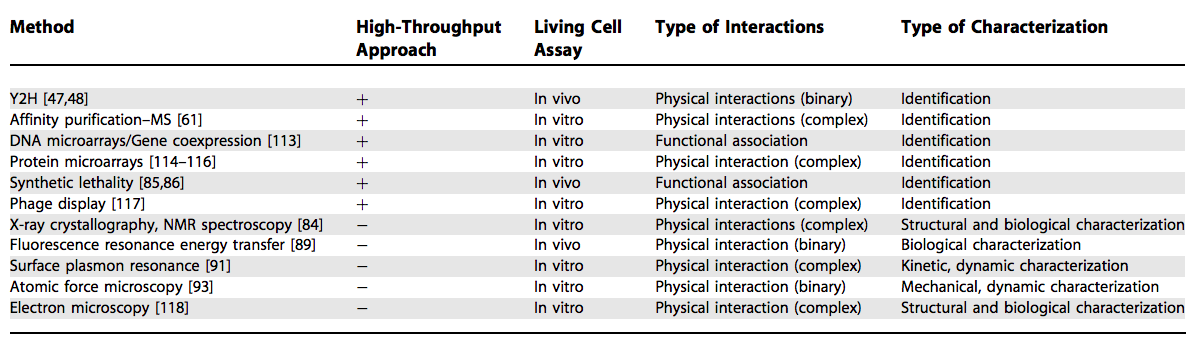
\includegraphics[ width = 16cm]{img/experimental_PPI_identification.png}
\caption{Experimental methods for PPI identification (From \cite{shoemaker2007deciphering}). High-throughput methods are marked with + in the second column. The fourth column shows whether the method on physically interacting proteins in a complex (‘‘complex’’) or only pairwise interactions (‘‘binary’’).   \label{table_experimental_ppi_pred}}
\end{center}
\end{table}

In general, based on the input, computational methods can be classified into two categories: sequence based and structure based \cite{zhang2018review}. Sequence based methods are faster and more universal because not all proteins have structures available. 

\subsubsection{SigProd}
\subsubsection{PIPE}
\subsubsection{Ding's}
\section{Methods}
\subsection{SPRINT Overview}
\subsection{Training Data Preparation}
\subsection{Detecting Similarities}
\subsubsection{Seed representations}
\subsubsection{Storing sub-sequences}
\subsubsection{Hash table and hash function}
\subsection{Predicting Interactions}
\subsubsection{Post-processing similarities}
\subsubsection{Scoring function}
\subsubsection{Fast prediction}
\subsection{Implementations}
\section{Results}
\subsection{Datasets}
\subsection{Evaluation Scheme}
\subsection{Comparative Analysis on Park \& Marcotte’s Datasets}
\subsection{Comparative Analysis on Seven Human Datasets}
\subsection{Comparative Analysis on Human Interactome Prediction}
\subsection{Availability}
\section{Conclusion}
% \section{Basic Theorems}
% \begin{theorem}
%  $e^{i\pi} = -1$ \label{eipi}
% \end{theorem}